\chapter{Phonemized CHILDES: A Phonemic Multi-Lingual Corpus of Child-Directed Speech}

\rough{Single paragraph introduction to chapter}

\section{Introduction}
\label{sec:dataset-intro}

Language modelling is a core task in NLP that involves learning the structure of language by making predictions of individual language units given a context. There is considerable variation in how the task is approached, whether it be the granularity of the language unit being predicted (such as words, characters or subwords), the model being used (n-gram models, RNNs, transformers) or the objective being optimised (such as next-token prediction or masked language modelling). In all cases, a dataset is required from which the distributed statistics of the language can be extracted.

In this thesis, I explore the specific variation of langugage modelling task where the language unit is the phoneme, the model used is a transformer and the objective is next-token prediction. The first challenge, and the topic of this chapter, is to source a suitable dataset for this task, given that this variation of language modelling is under-studied. I require a dataset that is not only representative of child input across many languages to support the analytical experiments in Chapters 5 and 6, but one that can also aid in addressing the modelling challenges presented in Chapter 4. 

I begin this chapter by discussing the properties to consider when selecting a dataset for a particular language modelling task, the specific properties I require for the experiments carried out in this thesis, and the range of existing datasets that may meet these requirements (\cref{sec:dataset-background}). After concluding that no such dataset exists, I propose \textbf{automatic phonemization} as a method for converting orthographic datasets to a phonemic format and present \corpusphonemizer, a tool I developed to facilitate the creation of large phonemic datasets (\cref{sec:dataset-corpus-phonemizer}). I then describe the use of this tool to create \phonemizedchildes, a dataset consisting of child-directed speech from 31 languages, meeting all requirements for the work in this thesis (\cref{sec:dataset-phonemized-childes}). Finally, I explore the limits of automatic phonemization by comparing human-transcribed phonemic data to the phonemic data produced by my tool (\cref{sec:dataset-limitations}).

%One important property is the \textbf{granularity} of the data. Language models can be trained on words, characters, subwords or phonemes. Phonemic data is useful for studying the structure of language, as it is more closely related to the underlying phonological structure of the language. However, phonemic data is not as readily available as orthographic data, and so datasets containing phonemic transcriptions are less common.

%The main property concerning modern application-driven language modelling is \textbf{scale} --- very large transformer-based language models trained for chat-based appliations are extremely data hungry, and datasets such as The Pile and CommonCrawl have been developed to expose these models to trillions of words of English. Even in smaller applications involving large language models, previous language modelling datasets used for n-gram modelling such as The Brown Corpus (containing one million words) are no longer sufficient in scale.

%Another important property is the \textbf{domain} --- if the language model is being used to model a particular domain, the data should be representative of that domain. This is often important for applications surrounding that domain. For example, the Switchboard Corpus, containing transcriptions of telephone conversations, was originally collected to improve n-gram language modelling for speech recognition software\todo{check this}. It can also be important for analytical purposes, such as using a dataset consiting of child-directed speech when studying language acquisition.

%A third property is the \textbf{modality} of the data. Language models can be trained on text, speech or both. Speech models are often trained on phonemes, the smallest unit of sound in a language, which can be useful for applications such as speech recognition or synthesis. Text models are often trained on orthographic text, which is more readily available and easier to process. However, phonemic data is often more useful for studying the structure of language, as it is more closely related to the underlying phonological structure of the language.

%A final property is the \textbf{language} of the data. Language models are often trained on English, due to the availability of data and the dominance of English in research. However, it is important to consider the properties of other languages, especially when studying the properties of language in general or when studying language acquisition. For example, the properties of English child-directed speech may not be representative of child-directed speech in other languages.

\section{Background}
\label{sec:dataset-background}

There are several dimensions to consider when determining the suitability of a dataset for a particular language modelling task, often determined by the analytical or downstream use of the language model being trained. The first dimensions is the \textbf{modality} of the dataset. Language models can be trained on a diverse range of data representations, including written text, phonemic transcriptions, images and continuous audio\todo{possibly cite examples for each of these}. Often the modality should match the downstream purpose of the language model (whether to solve additional tasks or study linguistic properties) and it is difficult to train a language model with one modality and apply it to another \citep{suvarna-etal-2024-phonologybench,lavechin}.

The \textbf{domain} of the dataset should also be representative. Some datasets are collected to match one specific domain. For instance, the Switchboard corpus was originally collected to improve n-gram language modelling for speech recognition software \citep{godfrey1992switchboard}. In other cases, datasets consist of many domains, represent a broad range of language use in order to improve general-purpose language models. An early benchmark for n-gram language modelling research was the Brown Corpus, which consisted of 1 million words across various genres, such as news, fiction, reviews and essays\citep{francis1979brown}.

Another important consideration is the \textbf{scale} of the dataset. This is typically determined by the size of model being used for the task. The Brown Corpus may have been sufficient to train n-gram models but modern transformer-based architectures are extremely data-hungry, often trained on datasets containing trillions of words \citep{elazar-2024-redpajama}, despite the diminishing returns \citep{kaplan2020scaling}. Examples of such datasets include The Pile \citep{pile} or CommonCrawl\footnote{\url{https://commoncrawl.org}} which also aim to include a diverse range of domains in order to improve the generalisation of the model for downstream tasks.

Finally, the \textbf{language} of the dataset also depends on the eventual use of the language model. Many of the largest datasets only exist in English due to the availability of data and the dominance of English in NLP research, but if the purpose of the language model is to build translation systems or facilitate the the cross-lingual comparison of language properties, multi-lingual datasets are required.

Within each of these dimensions there are many datasets to choose from. However, when considering a particular instance of the language modelling task, certain properties do not always align. This is particularly the case when considering the \textbf{scale} of datasets. Very large datasets are required to train transformer-based architectures, but it is difficult to satisfy \textbf{domain}, \textbf{modality} and \textbf{language} requirements when the scale of datasets reaches trillions of words. The very largest datasets only exist due to the practice of web-scraping \citep{bansal-2022-datascaling} and so are typically only representative of written text and particular domains. This practice also leads to a skew towards English data, as English continues to account for over 50\% of the text on the internet \citep{ebbertz2002, danet2007multilingual, DataReportal2024}.

This creates a challenge for the work in this thesis, as I require sufficient data to train transformer-based language models, but I also require the data to have a phonemic modality. Finding datasets that meet these two requirements alone is already a challenge, but in order to support the analytical experiments in Chapter 5 and 6, I also require the dataset to be multi-lingual and have a domain representative of child-directed speech. This is a unique set of requirements that is not met by any existing dataset. However, \textbf{automatic phonemization} can be used to convert orthographic datasets to phonemic datasets, and this can be used to create a dataset that meets all requirements for the work in this thesis.

In this section, I begin by giving further background into these specific requirements (\cref{sec:dataset-requirements}). I then compare these requirements against existing datasets, finding that none match all of the requirements (\cref{sec:dataset-existing}). I then explore the use of automatic phonemization to convert orthographic datasets to phonemic datasets, which could be used to solve the \textbf{phonemic} constraint (\cref{sec:dataset-phonemization}). Finally, I present the specific phonemic representation I use in this thesis (\cref{sec:dataset-phoneme-streams}).

%For example, very large transformer-based language models trained for chat-based applications mostly rely on \textbf{scale}, often requiring datasets with trillions of words such as The Pile \citep{pile} or CommonCrawl\footnote{\url{https://commoncrawl.org/}} to meet their data-hungry nature. These models also aim for diverse \textbf{domains} to be included in the dataset so that the model can be exposed to a wide range of language phenomena, whereas other language models may aim to model a single domain. For example, the Switchboard Corpus was originally collected to improve n-gram language modelling for speech recognition software. The \textbf{language} of the data is another crucial factor: many of the largest datasets only exist in English due to the availability of data and the dominance of English in research, but if the purpose of the language model is to build translation systems or facilitate the comparison of the properties of different languages, multi-lingual datasets are required. Finally, the \textbf{modality} of the data is important to consider. Language models can be trained on text, speech or both. Speech models are often trained on phonemes, the smallest unit of sound in a language, which can be useful for applications such as speech recognition or synthesis. Text models are often trained on orthographic text, which is more readily available and easier to process.

\subsection{Requirements}
\label{sec:dataset-requirements}

I can now discuss the specific requirements for the dataset used in this thesis according to the \textbf{modality}, \textbf{scale}, \textbf{domain} and \textbf{language} of the data.

\paragraph{Modality:} Since the phoneme is the unit of language we are modelling, our first requirement is that the training data must have a \textbf{phonemic} representation. Phonemic representations can vary considerably in terms of the level of details (e.g. broad phonemic transcriptions or narrow phonetic transcriptions) as well as the alphabet used. The most comprehensive and widely used alphabet is the International Phonetic Alphabet (IPA) which includes a broad range of symbols for phonemes as well as diacritics to represent finer phonetic details. There are also alphabets that were created for specific languages, such as the Americanist Phonetic Notation for Native American languages and the Uralic Phonetic Alphabet for Uralic languages. Other languages such as the Speech Assessment Methods Phonetic Alphabet (SAMPA) \citep{wells1992standard} or the Kirschenbaum Phonetic Alphabet were developed as machine-readable alternatives to IPA, representing sounds with ASCII characters. There exist tables to easily convert between these alphabets, so the exact choice is not crucial. However, a phonemic representation is necessary to ensure that the model is learning the structure of language at the phonological level. \rough{Either explain differences between orthographic and phonemic data, or probably refer to chapter 1 or 2 where this is discussed in further detail.}

\paragraph{Scale:} In this thesis I use a transformer-based architecture for the language modelling task. It is clear from the scaling laws of neural language models that larger datasets are beneficial \citep{bansal-2022-datascaling} and transformer-based language models trained on the largest datasets available have demonstrated impressive linguistic capabilities \rough{citations here}. However, the purpose of the language models trained in this thesis is not to achieve high performance on application-driven benchmarks, but to study the properties of language. This means that the scale of the dataset is not as crucial as it would be for chat-based applications. The BabyLM workshop has demonstrated that language models can achieve good performance on a range of linguistic tasks when the scale of the training data is limited to 10-100 million words, mimicking the linguistic experience of a 13-year-old \citep{warstadt-2023-babylm-findings}, but this is still considered \textbf{large} in the context of phonemic datasets. The question of what quantity of data is required for a language model to learn specific properties of language is still an open question and is under-studied in the phonemic domain. This question is addressed in Chapter 4, requiring a dataset that is still in the order of millions of words in order to carry out this analysis.

\paragraph{Domain:} In order to investigate the spoken properties of language, the dataset being used in language modelling should be sourced from a \textbf{speech} domain. This is closely linked with the phonemic modality of the data, although many speech-based datasets are represented as audio files or as orthographic transcriptions. Speech datasets also vary considerably according to how naturalistic the data is. For instance, audio book datasets are more representative of written language use than spoken language use, which is often more informal, with more disfluencies, repetition and incomplete sentences \rough{[citation]}. It is important to match the domain we are seeking to model and language models trained on clean audio book data have demonstrated very different characteristics when compared to recordings of naturalistic, spontaneous speech \citep{lavechin}\todo{maybe cut this sentence since we mention it below}. Naturalistic speech is also more representative of the input that children acquire langauge from, and child-directed speech has unique properties such as ... \rough{[examples and citation]}. Given this, the dataset should also be \textbf{child-directed} for the simulation experiments in Chapter 6. 

\paragraph{Language:} Finally, I require the dataset to be \textbf{multilingual} both for the cross-lingual phonological analysis of languages carried out in Chapter 5 and also to support the acquisition study in Chapter 6. When testing hypotheses to do with the structure of language and the learnability of language, it is important to test the hypothesis on as many languages as possible and across as many language families as possible. Every language has a different structure, so while one model may work well for one language, it may not on another. This is especially important for acquisition experiments where language-independent mechanisms are being proposed. \rough{Citations and tidy this up further}

These properties are motivated by the work in this thesis and are not necessarily required for all language modelling tasks. If the purpose of the language model is only to examine the the phonological structure of language, we only require the data be \textbf{large} and \textbf{phonemic}. Comparing the phonological properties of language also does not necessarily require the data to come from \textbf{child-directed} sources, although this is the particular domain I examine in this work. Similarly, for experiments studying a particular language, the dataset does not necessarily need to be \textbf{multilingual}, although having a single multilingual dataset does facilitate many monolingual studies.

A final property that is not mentioned here is the \textbf{parallel} nature of the data. Parallel data is often used in translation tasks, where the model is trained to predict the target language given the source language. In this thesis, we are not training a translation model, but it is useful to have parallel data for validation experiments. This is particularly useful when converting orthographic data to phonemic data, as it allows us to compare the output of the automatic phonemization process to human-transcribed phonemic data.

\subsection{Existing datasets}
\label{sec:dataset-existing}

There are several existing datasets that meet some of the requirements outlined above, but there are often trade-offs. I describe these further below and summarise them in \cref{tab:dataset-requirements}.

Typical datasets for pre-training LLMs such as The Pile tend to only meet the size requirement, as they primarily consist of English written text. Other pre-training datasets are multilingual, such as the C4 dataset which contains text from 108 languages \citep{raffel2020exploring}, but such datasets do meet the domain or representation requirements.

In order to find phonemic datasets we must instead look to datasets that were collected for speech recognition research. The GlobalPhone database, for instance, is a large, multilingual dataset with phonemic transcriptions designed to support the deployment of multilingual speech-based applications \citep{schultz2013globalphone}. It is also a \textbf{parallel} dataset, containing both audio, phonemic transcriptions and pronunciation dictionaries to facilitate orthographic analysis. Similarly, Common Voice \citep{ardila-etal-2020-common} consists of over 2,500 hours of audio across 38 languages, but does not include phonemic transcriptions. A limitation of both corpora is that they do not contain naturalistic speech. Instead, speech is elicited from the participants. For GlobalPhone, speakers given just 100 sentences from national newspaper articles to read aloud, and for Common Voice, speakers were provided individual, grammatically correct sentences to record themselves reading. GlobalPhone is also behind a paywall, which may limit its use in research. 

Elicited speech corpora are frequently used in speech processing research because currating the sentences allows researchers to control for phonetic converage, speaker variability and contextual diversity \citep{lamel1989speech}. For instance, the TIMIT acoustic-phonetic database contains 2342 sentences spoken by 630 speakers across English regions and dialects, with audio aligned to detailed phonetic transcriptions \citep{garofolo1993darpa}. Such datasets have also been used for training language models. For instance, LibriSpeech --- which contains 1000 hours of read audibooks from the LibriVox project \citep{panayotov2015librispeech} --- is used as training data for the Zero Resource Speech Challenge, which aims to develop unsupervised methods for discovering linguistic units from speech \citep{dunbar_self-supervised_2022}. However, the clean and elicited nature of the data does not reflect spoken language use, and provides an unrealistic training signal for unsupervised audio-based LLMs \citep{lavechin}. LibriSpeech also does not contain phonemic transcriptions, although Libri-Light, a derived versions of the dataset, has provided phonetic alignments \citep{Kahn_2020}.

Naturalistic speech corpora are more representative of spoken language use, but are often more challenging to collect, often leading to a trade-off between size and phonemic detail. For instance, Switchboard \citep{godfrey1992switchboard} and the Fisher corpus \citep{cieri2004fisher} are both large datasets consisting of recorded telephone conversations, but are only orthographically transcribed. The Buckeye corpus, which contains naturalistic speech from 40 English speakers does have parallel orthographic, phonetic and audio data, but does not meet the size requirement, only containing 300,000 words \citep{pitt2007buckeye}. One corpus that seems to bridge the gap is Audio BNC which contains 7.5 million words of naturalistic speech, provided as audio files aligned with phonemic transcriptions \citep{coleman2012audio}. Audio BNC was derived from the British National Corpus (BNC) which contains 100 million words of text \citep{bnc2007} reflecting a range of British English language use at the end of the 20th century. The spoken portion of BNC consisted of 10 million words of naturalistic speech transcribed orthographically, the majority of which was aligned with the original tape recordings to create Audio BNC as part of the Mining a Year of Speech project \citep{coleman2011mining}. Another large corpus with phonemic transcriptions which is also multilingual is the Babel corpus, consisting of aligned audio, word-level and phoneme-level transcriptions of conversational speech across 22 minority languages \citep{gales2014speech}. However, as with GlobalPhone, the corpus is not distributed with an open license. 

Although many of the datasets described above have met the naturalistic speech requirement, none have fulfilled the \textbf{child-directed} requirement. The \emph{de facto} repository for language acquisition data is the Child Language Data Exchange System (CHILDES) database \citep{macwhinney1985child}. CHILDES was developed with the aim of preserving and standardising data used for child language development research and later grew into the TalkBank project, which now contains over 1.4TB of transcript data and 5TB of associated media data across several ``banks'', each focusing on a particular type of spoken language \citep{macwhinney_understanding_2019}. CHILDES is now a very large database, containing naturalistic child-adult interactions in over 40 different languages. It is a valuable resource for research on child language development, allowing past corpora to be used to answer new research questions, many of which could not have been ``remotely envisioned'' when the corpora were originally collected \citep{bernstein_ratner_augmenting_2024}. 

CHILDES meets the majority of the requirements for the work in this thesis, as a multilingual corpus of naturalistic child-directed speech. CHILDES also may be sufficiently large for training transformer-based language with the North American English portion alone containing over 20 million words, of which 7 million words are child-directed. This portion has been used to train large language models in the past \citep{huebner-etal-2021-babyberta} but the other languages in the database contain fewer words. Whether these sections are sufficient for training large language models is an open question which I address in Chapter 4. The only limitation of CHILDES is that the data is primarily orthographically transcribed and so fails to meet the primary requirement. The PhonBank section of TalkBank does contain phonemic transcriptions but primarily for child-produced speech, with fewer than 100 adult utterances transcribed phonemically. 
\todo{maybe mention homebank for longitudinal data}

Finally, there exist some corpora that are child-directed but are not speech-based, such as the children's stories in Project Gutenberg \citep{gerlach2018standardizedprojectgutenbergcorpus}. This dataset makes up a portion of the pre-training dataset used for the BabyLM workshop, which was designed to mimick the linguistic experience of a 13-year-old both and consists of 100 million words. By combining data from multiple corpora including CHILDES, BNC and Switchboard, the BabyLM pre-training dataset aims to be representative of the input a child receives while also being sufficiently large \citep{choshen-et-al-2024-callforpapers-babylm2}. However, although 58\% of the data is derived from speech transcripts and 70\% of the data is child-directed, only the 29\% of the data (the CHILDES portion) is naturalistic child-directed speech. The remaining speech data is adult-directed and the remaining child-directed data consists of written stories or simplified Wikipedia articles. The dataset is also not phonemic or multilingual, but the dataset is still a useful resource for training transformer-based language models on relatively smaller corpora.

% \begin{table}[t]
%     \centering
%     \begin{tabular}{c||cc|c|cc|c}
%     %\toprule
%         % Rotate text using \rotatebox from graphicx package
%         & \multicolumn{2}{c|}{\textit{Modality}} & \multicolumn{1}{c|}{\textit{Scale}} & \multicolumn{2}{c|}{\textit{Domain}} & \textit{Language} \\
%         & \footnotesize{\textbf{Phonemic}} & \footnotesize{\textbf{Parallel}} & \footnotesize{\textbf{Large}} & \footnotesize{\textbf{Speech}} & \footnotesize{\textbf{Child-Directed}} & \footnotesize{\textbf{Multilingual}} \\
%         \hline
%         GlobalPhone & \cmark & \cmark & \cmark & (\cmark) & \xmark & \cmark \\
%         CHILDES & \xmark & \xmark & \cmark & \cmark & \cmark & \cmark \\
%         AudioBNC & \cmark & \cmark & \cmark & \cmark & \xmark & \xmark \\
%         BabyLM & \xmark & \xmark & \cmark & (\cmark) & (\cmark) & \xmark \\
%         \hline
%         Phonemized BabyLM & \cmark & \cmark & \cmark & (\cmark) & (\cmark) & \xmark \\
%         Phonemized CHILDES & \cmark & \cmark & \cmark & \cmark & \cmark & \cmark \\
%     \end{tabular}
%     \caption{A summary of the properties of existing datasets that are used in this thesis.}
%     \label{tab:dataset-requirements}
% \end{table}

\begin{table}[t]
    \centering
    \footnotesize
    \begin{tabular}{l||cc|c|cc|c}
    \toprule
        % Rotate text using \rotatebox from graphicx package
        & \multicolumn{2}{c|}{\textit{Modality}} & \multicolumn{1}{c|}{\textit{Scale}} & \multicolumn{2}{c|}{\textit{Domain}} & \textit{Language} \\
        {\textbf{Dataset}} & {\textbf{Phonemic}} & {\textbf{Parallel}} & {\textbf{Large}} & {\textbf{Speech}} & {\textbf{Child-Directed}} & {\textbf{Multilingual}} \\
        \midrule
        The Pile & \xmark & \xmark & \cmark & \xmark & \xmark & \xmark \\
        C4 & \xmark & \xmark & \cmark & \xmark & \xmark & \cmark \\
        GlobalPhone & \cmark & \cmark & \cmark & (\cmark) & \xmark & \cmark \\
        Common Voice & \xmark & \xmark & \cmark & (\cmark) & \xmark & \cmark \\
        TIMIT & \cmark & \cmark & \xmark & (\cmark) & \xmark & \cmark \\
        LibriSpeech & \xmark & \cmark & \cmark & (\cmark) & \xmark & \xmark \\
        Libri-Light & \cmark & \cmark & \cmark & (\cmark) & \xmark & \xmark \\
        Switchboard & \xmark & \cmark & \cmark & \cmark & \xmark & \xmark \\ 
        Fisher & \xmark & \cmark & \cmark & \cmark & \xmark & \xmark \\
        Buckeye & \cmark & \cmark & \cmark & \cmark & \xmark & \xmark \\
        AudioBNC & \cmark & \cmark & \cmark & \cmark & \xmark & \xmark \\
        Babel & \cmark & \cmark & \cmark & \cmark & \xmark & \cmark \\
        CHILDES & \xmark & \xmark & \cmark & \cmark & \cmark & \cmark \\
        Gutenberg Stories & \xmark & \xmark & \xmark & \xmark & \cmark & \xmark \\ 
        BabyLM & \xmark & \xmark & \cmark & (\cmark) & (\cmark) & \xmark \\
        \midrule
        Phonemized BabyLM & \cmark & \cmark & \cmark & (\cmark) & (\cmark) & \xmark \\
        Phonemized CHILDES & \cmark & \cmark & \cmark & \cmark & \cmark & \cmark \\
        \bottomrule
    \end{tabular}
    \caption{A summary of the properties of existing datasets that are used in this thesis.}
    \label{tab:dataset-requirements}
\end{table}

\todo{check whether switchboard has phonemes and check gutenberg properties in table}

\rough{Clearly none match all the requirements we want for the work in this thesis, a good solution is \textbf{automatic phonemization} to convert CHILDES and BabyLM Pre-training data. Talk about how some even fully sythesise speech and then use ASR to get phonemic data. E.g. \citep{zissman1994automatic} with switchboard}

Two approaches to getting phonemes: 1) use ASR to get phonemes from audio data, 2) use automatic phonemization to convert orthographic data to phonemic data. The latter is the approach I take in this thesis.
Some people have trained phonemic language models by first using ASR on audio data to generate phonemes, then training a language model on these phonemes \citep{zissman1994automatic}.

In general, there are trade-offs between the properties of the datasets. The main challenge seems to be finding \textbf{phomemic} datasets that are sufficiently \textbf{large} for training transformer-based language models. It is then even more challenging to find datasets that also match the particular domain and language requirements of this thesis. If CHILDES were available in a phonemic format, it would be a suitable dataset for this work. One solution to this problem is to use \textbf{automatic phonemization} to convert orthographic datasets to a phonemic format. This is the approach I take in this thesis.

\subsection{Automatic phonemization}
\label{sec:dataset-phonemization}

\rough{Argue why automatic phonemization is a good approach. Discuss the way this has been approached in the past. Mention the benefits and potential limitations, mention that we will tackle this in the last section. Say but first we need to define our phoneme stream representation...?}

\subsection{Phoneme streams}
\label{sec:dataset-phoneme-streams}

\rough{Describe phoneme stream representation as a useful way to store phonemes. Referencing past phonemic representations and how it's useful to do space-separation due to multi-character symbols in IPA. Mention word boundaries also included and give an example}

\subsection{Summary}
\label{sec:dataset-background-summary}

\rough{Summarise background.}

\section{Corpus Phonemizer}
\label{sec:dataset-corpus-phonemizer}

In order to address the challenges of automatically converting orthographic datasets to phonemic streams, I developed \corpusphonemizer,\footnote{\url{https://github.com/codebyzeb/Corpus-Phonemizer}} a suite of tools and scripts for converting datasets from an orthographic representation to the phoneme stream representation.

The primary tool in the suite is a command-line application \texttt{corpus\_phonemizer.py} which takes orthographic text as input and converts it to phonemes. The tool supports many languages by leveraging backend transliteration tools which can be selected by the user, each of which provides a different set of language codes (see \cref{sec:dataset-transliteration-tool-backends}).

A crucial component of the tool is the use of \emph{folding dictionaries} to ensure that the set of phonemes produced by the backend transliteration tool for a particular language matches a standard phonemic inventory for that language. This validation step is important, \todo{expand on this}. It is also important to ensure that when designing the folding dictionaries, a consistent methodology is used. In order to support my multi-lingual experiments, I created folding dictionaries for 31 language codes. This process is described in \cref{sec:dataset-folding}.

The tool is versatile, supporting many options for ease-of-use when preparing corpora. Despite the tool's utility, there are still limitations to using an automated tool for creating phonemic transcriptions from orthographic text. I give example usage in \cref{sec:dataset-usage} and discuss these limitations further in \cref{sec:dataset-limitations}.

%Besides the command-line application, the \corpusphonemizer suite also contains scripts dedicated to preparing the specific datasets used in this thesis. These include:
% \begin{itemize}
%     \item The Phonemized CHILDES dataset 
%     \item The BabyLM pre-training dataset
%     \item The BLiMP, BLiMP Supplement and GLUE evaluation sets
%     \item The British National Corpus (BNC)
% \end{itemize}
% Phonemized CHILDES is a large corpus of child-directed speech across 31 languages. I describe the creation of this dataset in \cref{sec:dataset-phonemized-childes}. The other datasets are in English and follow a similar process so I do not go into detail on their creation.

\subsection{Transliteration tool backends}
\label{sec:dataset-transliteration-tool-backends}

In order to convert orthographic text to phonemes, I leverage four transliteration tools, each of which supports a different set of languages. The tools use different approaches for different languages, including rule-based transliteration and dictionary pronunciations. In order to ensure a consistent output, I create a custom wrapper for each tool.

\paragraph{\texttt{phonemizer}:}
Phonemizer \citep{Bernard2021} is a python library that supports the automatic phonemization of text in many languages. It allows the user to select from one of four backends, each of which have different capabilities. By default, I use eSpeak \citep{Dunn2019}, an open-source speech synthesizer which supports over one hundred languages and outputs phonemes in IPA. This synthesizer uses a combination of handwritten rules and pronunciation dictionaries for each language it supports. Besides supporting many languages, it also supports many accents (such as Scottish English or Lancaster English) but only for a few languages besides English. For Japanese text written in Romanji, I instead use \texttt{phonemizer} with the Segments \citep{robert_forkel_2019_3549784} backend, which uses simple grapheme to phoneme mapping (Romanji has very simple pronunciation rules and is not supported by eSpeak).\footnote{\texttt{phonemizer}'s segments dictionary for Japanese was actually missing an entry to map `s' to /s/ but I was able to add this to their codebase and become a contributor of their project.}

\paragraph{\texttt{epitran}:}
Epitran \citep{Mortensen-et-al:2018} is similar to \texttt{phonemizer}, supporting the automatic phonemization of text across many languages with a particular focus on low-resource languages. For English it uses the Flite Speech Sythesis System \citep{black2001flite} as a backend and for Simplified and Traditional Chinese it uses the CC-CEDict dictionary\footnote{\url{https://cc-cedict.org}} but for the remaining 92 languages supported, it uses greedily-interpreted grapheme-to-phoneme maps augmented with context-sensitive pre-processor and post-processor rewrite rules. These are implemented using CSV files to facilitate the addition of new languages. The tool also supports alternative scripts for certain languages, such as Pinyin for Mandarin.

\paragraph{\texttt{pinyin\_to\_ipa}:} pinyin-to-ipa \citep{taubert_2024_pinyin-to-ipa_2024} is a python library for converting Mandarin written in pinyin to IPA using a few contextual grapheme-to-phoneme maps. The phoneme inventory is based on the phonology of Mandarin as described by \cite{lin2007sounds} and \cite{duanmu2007phonology} and tone markers are attached to the vowel of the syllable, rather than the end of the syllable. The tool only converts individual pinyin syllables, so my wrapper first splits the input into syllables (carefully maintaining word boundaries) before using the tool to convert each syllable to IPA.

\paragraph{\texttt{pingyam}:} Pingyam\footnote{\url{https://github.com/kfcd/pingyam}} is a table storing the conversion relationships between the various romanization systems of Cantonese, based on data from the Open Cantonese Dictionary.\footnote{\url{https://www.kaifangcidian.com/han/yue/}} Since the table also contains IPA, my \texttt{pingyam} wrapper uses the table to convert from the Jyutping romanization scheme to IPA by splitting the input text into syllables, finding each syllable in the table and outputting the corresponding IPA transcription. The table places tone markers after the syllables, so I implemented a utility to move the tone marker to be attached to the vowel of the syllable instead.

\subsection{Phoneme inventory validation}
\label{sec:dataset-folding}

For a given backend tool and language code, Corpus Phonemizer will convert orthographic text into phonemes. The specific set of phonemes produced will be drawn from a vocabulary determined by the specific rules or pronunciation dictionaries created for that backend and language code. Since these tools are open-sourced, and since the exact \textbf{phoneme inventory} of languages are often up for debate, it is important to ensure that the phoneme inventory produced by the backend-language choice is consistent with established phoneme inventories for that language.

For each backend-language pair used in this thesis, I examine the set of phonemes produced and compare them to the phoneme inventories for that language in \phoible, a database containing phoneme inventories extracted from source documents and tertiary databases for 2186 distinct languages \citep{phoible}. The database also contains phonetic feature information for each phoneme which is useful for comparing phonemes within an inventory. As there are often multiple inventories in \phoible for each language, I find the inventory that best matches the output phoneme set according to the number of phoneme types, the number of consonants, the number of vowels and the number of diphthongs.

Once the best inventory has been found, I use a process called \emph{folding} to align the output phoneme set with the inventory and correct errors in the output. Folding involves the construction of a look-up table (a \textbf{folding map}) which is applied to the output of the backend transliteration tool. There are several error types that can be solved using the folding map in order to align the phoneme sets, as detailed in \cref{tab:transcription-errors}. The most common of these are \textbf{one-to-one} errors, instances where the backend transliteration tool outputs a particular Unicode string for a specific phoneme but the inventory lists a different string, and so a simple one-to-one mapping can correct this. For example, the \texttt{phonemizer} backend with the \texttt{ja} language code (Japanese) outputs the tied characters \ttipa{\|c{ts}} as one of the phonemes, but the Japanese inventory we match with uses \ttipa{ts} instead. Another example is given in the top row of \cref{tab:transcription-errors}. These mappings that do not change the information-theoretic properties of the output (since the character(s) we map to do not already exist in the output) and only serve to match the symbols used in the inventory so that their phonetic features stored in \phoible can be used in further analyses.

\begin{table}[t]
    \centering
    \scriptsize
    \begin{tabular}{p{0.32\textwidth}p{0.26\textwidth}p{0.32\textwidth}}
    \toprule
        \textbf{Error type} & \textbf{Consequence} & \textbf{Example} \\
        \midrule
        \textbf{One-to-one:} The backend uses one symbol for a phoneme but the inventory lists a different symbol for that phoneme. & The one-to-one mapping does not change the number of types or tokens in the output. & \texttt{phonemizer} with language code \texttt{sv} (Swedish) outputs \ttipa{n} but the matching inventory uses \ttipa{\|[n}.\\
        \midrule
        \textbf{Many-to-one:} The backend produces two different phonemes that should only map to a single phoneme in the inventory. & The many-to-one mapping reduces the number of phoneme types. & \texttt{phonemizer} with language code \texttt{pt} (Portuguese) outputs both \ttipa{\*r} and \ttipa{r} but the matching inventory only lists \ttipa{K}.\\
        \midrule
        \textbf{Consonant merging:} The backend outputs two symbols for a consonant that should be written as a single phoneme. & The mapping merges the pair of consonants, reducing the number of phoneme tokens produced. & \texttt{epitran} with language code \texttt{srp-Latn} (Serbian) outputs the sequence \ttipa{d Z} but these are should be written as a single phoneme \ttipa{dZ}.\\
        \midrule
        \textbf{Vowel merging:} The backend outputs a pair of vowels as separate phonemes but they are typically analysed as a single diphthong. & The mapping merges the pair of vowels, reducing the number of phoneme tokens produced. & \texttt{pingyam} with language code \texttt{cantonese} outputs the sequence \ttipa{o u} but these are should be treated as a diphthong \ttipa{ou}.\\
        \midrule
        \textbf{Vowel splitting:} The backend outputs a diphthong that is not listed in the inventory and should be split into individual phonemes. & The mapping splits the pair of vowels, increasing the number of phoneme tokens produced. & \texttt{phonemizer} with language code \texttt{en-us} (American English) outputs \ttipa{aIU} as a single phoneme but this should be \ttipa{aI U}.\\
        \midrule
        \textbf{Phoneme duplication:} The backend outputs duplicate phonemes to represent long vowels or consonants or because of an error. & The mapping replaces the pair of phonemes with just one, reducing the number of phoneme tokens. & \texttt{phonemizer} with language code \texttt{et} (Estonian) outputs \ttipa{d d} but should output the long consonant \ttipa{d:}.\\
        \midrule
        \textbf{Diacritic error:} The backend incorrectly outputs the diacritic as a separate symbol instead of attaching it to the phoneme. & The mapping may change the number of phoneme types or tokens. & \texttt{phonemizer} with language code \texttt{ko} (Korean) outputs the diacritic for aspiration as \ttipa{h} instead of \ttipa{\super{h}} so sequences \ttipa{kh} and \ttipa{ph} are mapped to \ttipa{k\super{h}} and \ttipa{p\super{h}}.\\
        \midrule
        \textbf{Orthographic error:} Due to an invalid symbol in the orthographic text, the backend outputs an incorrect phoneme. & The contextual mapping changes the frequency statistics for the resulting phoneme, possibly reducing the number of phoneme types. & \texttt{epitran} with language code \texttt{hun-Latn} (Hungarian) outputs \ttipa{\^o} when the orthographic letter \textipa{\H{o}} is incorrectly written as \textipa{\^o} and so the phoneme is mapped to \ttipa{\o:}.\\
        \bottomrule
    \end{tabular}
    \caption{A list of errors that can occur during phonemization that can be fixed with a folding map but that may change the information-theoretic properties of the output.}
    \label{tab:transcription-errors}
\end{table}

The rest of the error types listed in \cref{tab:transcription-errors} are solved with mappings that are not necessarily one-to-one. These mappings may alter the number of output tokens or types by using a many-to-one mapping or by merging or splitting tokens. Since such a mapping will change the information-theoretic properties of the output, it is important that the they are linguistically motivated and carefully implemented. 

\subsubsection*{Folding map construction}

In order to construct the folding map for each backend-language pair, I run \corpusphonemizer on orthographic text for that language and compare the output set of phonemes $P_O$ to the phonemes in the closest inventory in \phoible $P_I$. I call the set of phonemes present in $P_O$ but not $P_I$ the ``unknown phonemes'' $U_K$ where $U_K = P_O \setminus P_I $ and the set of phonemes present in $P_I$ but not $P_O$ the ``unseen phonemes'' $U_S$ where $U_S = P_I \setminus P_O $. I then construct the folding map as follows:
\begin{enumerate}
    \item Find pairs $(k,s) \in U_K \times U_S$ that differ according to an accent or diacritic and obviously represent the same phoneme (determined by ruling out alternatives or examining where $k$ is produced in the output). Create a one-to-one mapping $k:s$ for each such pair, e.g. \ttipa{t} : \ttipa{t\super{h}}.
    \item Find pairs $(k,s) \in U_K \times U_S$ that clearly represent the same phoneme (determined as above) but may use entirely different symbols, possibly due to an alternative transcription scheme. Create a one-to-one mapping for each pair, e.g. \ttipa{a} : \ttipa{\ae}.
    \item For remaining items $k \in U_K$, determine whether these result from one of the other errors in \cref{tab:transcription-errors}. Carefully examine instances where $k$ is produced in the output and create a suitable mapping $k : p$ for some $p \in P_I$ to solve the error (the mapping may need to be contextual or include several characters, e.g. \ttipa{\textrhookschwa} : \ttipa{@ \*r} or \ttipa{U O} : \ttipa{w O}). 
    \item For remaining items $s \in U_S$, determine whether these result from one of the other errors in \cref{tab:transcription-errors}. Carefully examine instances where $s$ should be produced in the output and create a suitable mapping $k : s$ for some $k \in P_O$ to solve the error (the mapping may need to be contextual or include several characters). 
    \item Examine the output for cases of \textbf{phoneme duplication} and other errors that may not contain phonemes in $U_K$ or $U_S$ but could still be solved with the phoneme map and create suitable mappings.
\end{enumerate}

The goal is for $U_K = \{\} = U_S$ or equivalently $P_I = P_O$, i.e the set of phonemes produced by the tool perfectly aligns with the phoneme inventory in \phoible. This is not always possible, often there are a few remaining phonemes in $U_K$ and/or $U_S$. This can occur when no obvious mappings could be found in steps 1--4 above. For example, the \texttt{epitran} backend for German does not produce the phoneme \ttipa{Z} (it is ``unseen'') and none of the unknown phonemes seem to be a good match. Another possibility is that the output set of phonemes $P_O$ may not align well with any of the \phoible phoneme inventories and so the closest match may not include some of the unknown phonemes $k \in U_K$ despite being valid phonemes for that language and listed in other inventories. For example, the \texttt{epitran} backend for German produce the phonemes \ttipa{x} and \ttipa{5} which are not listed in the matching inventory but are listed in other established inventories for German. In other cases, the unknown phonemes may come from loan words (e.g. \ttipa{ts} for ``pizza'' in Portuguese). Finally, there are some cases where the output considerably disagrees with all of the \phoible inventories but is a valid phonemic analysis of the language according to other sources.

\todo[inline]{POSSIBLY MENTION THAT ENGLISH-US LANGUAGE CODE IS AN EXCEPTION BECAUSE WE HAVE TO MATCH BABYSLM}

In \cref{appendix:folding-dictionaries} I give the folding dictionary for each backend-language pair used in this thesis. I give the resulting phoneme inventory, describe the matching \phoible inventory and provide justification for any unknown or unseen phonemes.

\subsection{Usage}
\label{sec:dataset-usage}

%\rough{Describe overall usage of tool and how it can be used. Call forward to next section where it is used to produce the Phonemized CHILDES dataset. Briefly mention how it also used to create Phonemized BabyLM datset and can be used for evaluation data as well, calling forward to next chapter. Discuss limitations of the tool. Mention that folding maps optional}

The main usage of \corpusphonemizer is to use either use the command-line tool or equivalent python function call \texttt{phonemize\_utterances()} to convert orthographic text to a phonemic representation. The tool allows the user to select the backend and language code to use for phonemization and the command-line tool allows the text to be input/output from STDIN/STDOUt or to/from provided file paths. Additional options include \texttt{--keep\_word\_boundaries} to output a dedicated \texttt{WORD\_BOUNDARY} token between words and \texttt{--uncorrected} to skip the \textbf{folding} process and output the phonemes exactly as produced by the backend tool. 

\lstset{
    basicstyle=\ttfamily,
    columns=fullflexible,
    keepspaces=true,
    breaklines=true,
    showstringspaces=false,
    escapeinside={(*@}{@*)}
}
\begin{lstlisting}[float=th, breaklines=true,caption={Three examples of using Corpus Phonemizer's command-line tool to phonemize the line "hello there!". },label={listing:corpus-phonemizer}]
$ python corpus_phonemizer.py phonemizer --language en-us --keep-word-boundaries
hello there!
(*@\textipa{h @~l oU}@*) WORD_BOUNDARY (*@\textipa{D E \*r}@*) WORD_BOUNDARY

$ python corpus_phonemizer.py phonemizer --language en-us --uncorrected
hello there!
(*@\textipa{h @~l oU D E\*r}@*)

$ python corpus_phonemizer.py phonemizer --language en-us --input ortho.txt --output phonemes.txt --verbose --preserve_punctuation=True
DEBUG:src.wrappers.wrapper.PhonemizerWrapper:Initializing PhonemizerWrapper with language "en-us" and wrapper_kwargs "{'preserve_punctuation': True}"
DEBUG:src.wrappers.wrapper.PhonemizerWrapper:Using espeak backend with language code "en-us"...
DEBUG:src.wrappers.wrapper.PhonemizerWrapper:Applying folding dictionary for language code: "en-us".
\end{lstlisting}

I give three examples in \cref{listing:corpus-phonemizer}, all using the \texttt{en-us} language code with the \texttt{phonemizer} backend to phonemize the phrase ``hello there!''. The first example demonstrates how the tool can be used with input text provided in STDIN and output to STDOUT, with word boundaries maintained. The second example demonstrates how the folding step can be skipped, revealing that one of the errors corrected by the folding map is the incorrect merging of \ttipa{E\*r}. The final example shows how files can be passed to the tool and gives the output of the \texttt{--verbose} option. A full description of the tool's usage is given in \cref{appendix:corpus-phonemizer-usage}. 

\section{Phonemized CHILDES}
\label{sec:dataset-phonemized-childes}

Using \corpusphonemizer, I am able to address the orthographic limitation of CHILDES by converting the data to phonemes. The resulting corpus, which I call \phonemizedchildes, meets all of the data requirements that I presented in \cref{sec:dataset-intro}\todo{make sure this ref is correct}. In this section, I first describe the process of creating the dataset in \cref{sec:dataset-phonemized-childes-creation}. I then present an overview of the dataset in \cref{sec:dataset-phonemized-childes-overview}. Finally, I compare the properties of each language in the corpus in \cref{sec:dataset-phonemized-childes-analysis}.

\subsection{Dataset creation}
\label{sec:dataset-phonemized-childes-creation}

In order to prepare \phonemizedchildes, I created a utility tool called CHILDES Processor, hosted within the \corpusphonemizer suite. This tool provides the functionality needed to download and process corpora from CHILDES with the aim to create a single dataset with an individual section for each language. The tool has three modes:
\begin{itemize}
\item \textbf{Download:} This mode allows for individual corpora to be downloaded from CHILDES by specifying the section (e.g. ``Eng-NA'') and the name (e.g. ``Warren''). The corpus is saved as a CSV containing all the information in the CHILDES database for that corpus. If the name is not provided, all corpora are downloaded from the section and saved as a single CSV.
\item\textbf{Process:} This mode processes the downloaded CSV files and converts the orthographic utterances to phonemes using \corpusphonemizer according to a specified backend and language code. The tool also sorts the utterances by target child age and removes the child utterances so that only the child-directed utterances remain (this can be disabled). There are also several other optional features of the processing mode, such as the ability to restrict the maximum age of the target child and the ability to split the CSV into training set and a validation set.
\item\textbf{Extract:} This allows for an individual column from a processed CSV to be extracted and saved as a text file, useful for experiments where the entire CSV is not required.
\end{itemize}

Using this tool, I am able to prepare a section of my dataset for each language in CHILDES. This process is described in \cref{fig:dataset-phonemized-childes-prep}.

\begin{figure}[ht]
    \centering
    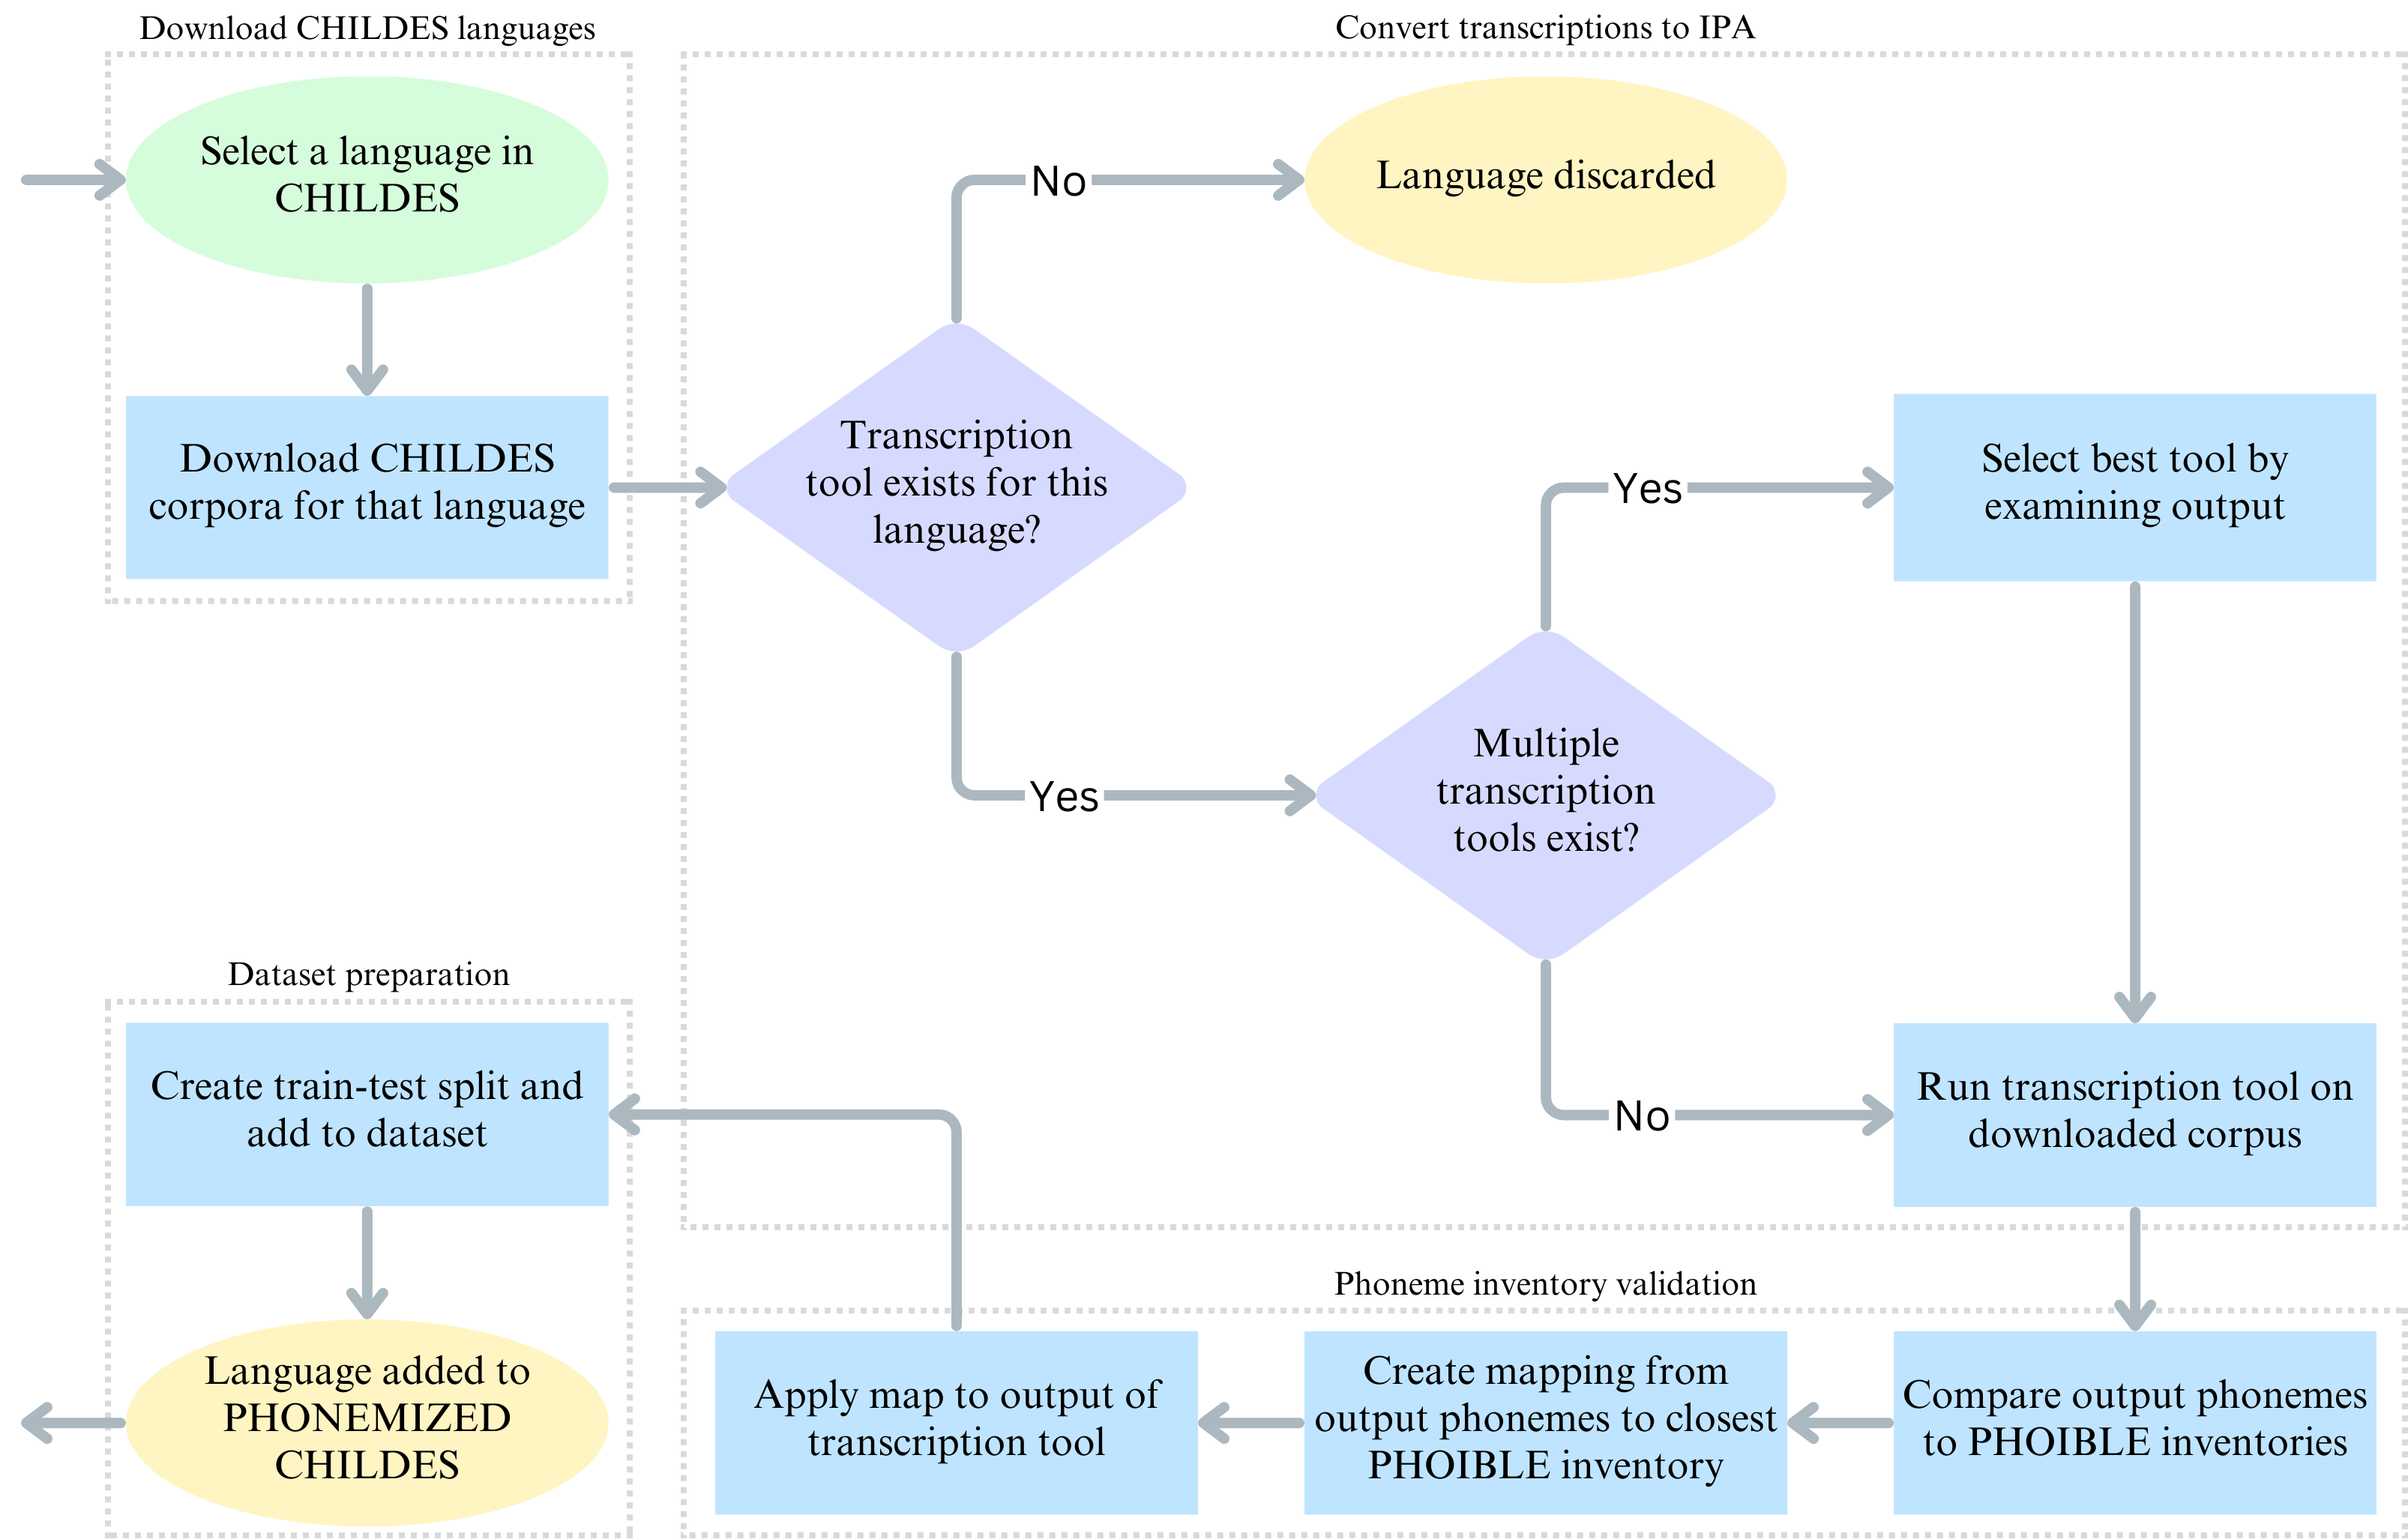
\includegraphics[width=0.9\linewidth]{Figures/13Dataset/data-prep.png}
    \caption{Data preparation pipeline for the \phonemizedchildes dataset.}
    \label{fig:dataset-phonemized-childes-prep}
\end{figure}

For each language hosted in CHILDES, I first use the \textbf{download} mode to individually download each corpus for that language that contain naturalistic child-directed utterances. I then assess whether \corpusphonemizer contains a backend and language code that supports that language. Unfortunately, this is not always the case. For instance, all Greek corpora in CHILDES are transcribed using a Latin script which is not supported by any of the backends in \corpusphonemizer. There are similar issues with Arabic, Hebrew, Thai, Georgian and Tamil.

If multiple backends support that language, I produce a transcription using each backend and carefully examine the output. The backend which produces a phonemic vocabulary which is closest to one of the phonemic inventories in \phoible is selected and is the backend for which I produce a folding map, as described in \cref{sec:dataset-folding}. I then run the \textbf{process} mode of CHILDES processor on all downloaded corpora for the language, using the selected backend and appropriate language code to phonemize the utterances (the folding map is automatically applied). This results in two CSV files for that language, a training set and a validation set containing 10,000 utterances.

Finally, I add the pair of CSV files to the \phonemizedchildes repository hosted on Huggingface. I then repeat this process for every language in CHILDES, resulting in 31 languages, as described in the next section. 

\subsection{Dataset overview}
\label{sec:dataset-phonemized-childes-overview}

The \phonemizedchildes dataset contains over seven million utterances of child-directed speech across 31 languages. Each language is available as a subset, with a `train' split containing the majority of the utterances downloaded from CHILDES and a `valid' split containing 10,000 utterances for validation purposes. An overview of each section is given in \cref{tab:dataset-phonemized-childes-sections}, detailing the corresponding CHILDES collection, the number of corpora downloaded, the backend and language code used with \corpusphonemizer to convert the corpora to phonemes and a numerical overview of the size of each section. Note that English is split into two sections to mirror the split present in CHILDES and Portuguese is split into two sections due to the phonological differences between Brazilian and Portugal Portuguese, the availability of language codes to phonemize the two, and the fact that the corpora are distinct within CHILDES.

\begin{table}[t]
    \centering
    \scriptsize
    \begin{tabular}{llllcccc}
        \toprule
        \textbf{Language} & \textbf{CHILDES Collection} & \textbf{Backend} & \textbf{Lang Code} & \textbf{Speakers} & \textbf{Utterances} & \textbf{Words} & \textbf{Phonemes} \\
        \midrule
        English (US)  & Eng-NA (44) & phonemizer & en-us & 2,692  & 1,645,797  & 7,096,724  & 22,107,530 \\
        English (UK)  & Eng-NA (14) & phonemizer & en-gb & 588  & 1,246,211  & 5,170,088  & 15,710,282 \\
        German  & German (10) & epitran & deu-Latn & 628  & 860,297  & 4,827,996  & 14,821,812 \\
        Japanese  & Japanese (9) & phonemizer & japanese & 329  & 557,215  & 1,773,816  & 7,100,307 \\
        Indonesian  & EastAsian/Indonesian (1) & epitran & ind-Latn & 389  & 534,525  & 2,122,372  & 6,369,459 \\
        French  & French (11) & phonemizer & fr-fr & 722  & 432,133  & 1,995,063  & 5,510,523 \\
        Spanish  & Spanish (18) & epitran & spa-Latn & 562  & 288,372  & 1,567,124  & 4,553,108 \\
        Mandarin  & Chinese/Mandarin (15) & pinyin\_to\_ipa & mandarin & 883  & 324,071  & 1,506,475  & 4,397,546 \\
        Dutch  & DutchAfricaans/Dutch (4) & phonemizer & nl & 78  & 261,938  & 1,106,865  & 3,585,608 \\
        Serbian  & Slavic/Serbian (1) & epitran & srp-Latn & 199  & 226,266  & 1,054,074  & 3,067,398 \\
        Estonian  & Other/Estonian (9) & phonemizer & et & 118  & 103,343  & 544,680  & 2,226,518 \\
        Cantonese  & Chinese/Cantonese (2) & epitran & yue-Latn & 81  & 147,673  & 651,392  & 1,824,730 \\
        Polish  & Slavic/Polish (2) & phonemizer & pl & 466  & 80,412  & 381,940  & 1,599,152 \\
        Swedish  & Scandinavian/Swedish (3) & phonemizer & sv & 32  & 85,299  & 396,800  & 1,242,615 \\
        Portuguese (Pt)  & Romance/Portuguese (3) & phonemizer & pt & 33  & 81,444  & 368,032  & 1,117,010 \\
        Korean  & EastAsian/Korean (3) & phonemizer & ko & 95  & 66,576  & 201,078  & 1,074,044 \\
        Italian  & Romance/Italian (5) & phonemizer & it & 92  & 57,542  & 264,479  & 996,701 \\
        Catalan  & Romance/Catalan (5) & phonemizer & ca & 159  & 56,588  & 248,999  & 839,462 \\
        Croatian  & Slavic/Croatian (1) & phonemizer & hr & 51  & 55,288  & 214,949  & 805,530 \\
        Welsh  & Celtic/Welsh (2) & phonemizer & cy & 65  & 55,871  & 269,295  & 785,569 \\
        Icelandic  & Scandinavian/Icelandic (2) & phonemizer & is & 15  & 50,657  & 197,519  & 751,804 \\
        Danish  & Scandinavian/Danish (1) & phonemizer & da & 25  & 48,976  & 192,527  & 579,972 \\
        Norwegian  & Scandinavian/Norwegian (2) & phonemizer & nb & 27  & 35,547  & 175,952  & 559,340 \\
        Basque  & Other/Basque (2) & phonemizer & eu & 150  & 36,614  & 135,866  & 565,633 \\
        Hungarian  & Other/Hungarian (3) & epitran & hun-Latn & 65  & 36,272  & 147,334  & 588,934 \\
        Romanian  & Romance/Romanian (2) & phonemizer & ro & 21  & 31,550  & 110,067  & 380,577 \\
        Portuguese (Br)  & Romance/Portuguese (2) & phonemizer & pt-br & 163  & 12,471  & 91,484  & 303,998 \\
        Irish  & Celtic/Irish (2) & phonemizer & ga & 20  & 18,256  & 88,388  & 278,558 \\
        Turkish  & Other/Turkish (2) & phonemizer & tr & 35  & 14,487  & 43,823  & 230,737 \\
        Quechua  & Other/Quechua (2) & phonemizer & qu & 7  & 13,425  & 33,102  & 204,692 \\
        Farsi  & Other/Farsi (2) & phonemizer & fa-latn & 23  & 13,467  & 28,080  & 115,089 \\
        \bottomrule
    \end{tabular}
    \caption{A breakdown of each language available as a subset of \phonemizedchildes. The bracketed number in the \textbf{CHILDES Collection column} refers to the number of corpora downloaded from that collection. The \textbf{Backend} and \textbf{Lang Code} columns refer to the \corpusphonemizer configuration used to convert utterances for that language to phonemes. The \textbf{Speakers} column refers to the number of unique speakers in each subset. The final three columns describe the size of the subset at three levels of analysis.}
    \label{tab:dataset-phonemized-childes-sections}
\end{table}
\todo[inline]{Possibly need to add the Phoible phoneme inventory information to this table, although perhaps that can be in the appendix.}

The dataset is hosted on Huggingface and can be loaded using Huggingface's \texttt{datasets} library \citep{lhoest-etal-2021-datasets} or downloaded directly. The dataset is stored as CSV files with one utterance per row, maintaining the structure of the CHILDES database. Both the original orthographic utterances and phonemized utterances are available, as well as many features imported from CHILDES, such as target child age, morpheme count, part of speech information, and the IDs of each utterance, transcript, corpus and collection. Within each section, the transcripts are sorted by target child age, to age-ordered curriculum learning experiments such as in the work of \citet{huebner-etal-2021-babyberta}.

\subsection{Corpus analysis}
\label{sec:dataset-phonemized-childes-analysis}

There is considerable variation in size between each subset in \phonemizedchildes. The largest subset is \textbf{English (US)} with over 1.6 million utterances and the smallest section is \textbf{Farsi} with only 13 thousand utterances. As these subsets reflect the number of utterances available for each language in CHILDES, which in turn come from individual corpora collected from acquisition research into that language, these differences give a sense of which languages are understudied in the field of acquisition, and the extent to which English dominates\todo{rewrite}. In this section, I compare each language in \phonemizedchildes according to their information-theoretic properties,   

\rough{A broad overview of the phonemic properties of each language within the corpus. A few experiments to justify why we use phonemes instead of letters, trying to highlight that phonemes are a more consistent representation for our purposes. Experiments include:
\begin{itemize}
    \item Information theoretic properties (Zipf's law, Heap's law, ratios, information rate, n-gram perplexities)
    \item Comparing phoneme properties to character properties (hypothesis: information rate more consistent across langugages when looking at phonemes rather than characters)
    \item Child vs adult speech (extract child utterances in CHILDES and compare MLU, word length etc)
    \item Child-directed vs adult-directed speech (compare CHILDES to BNC)
    \item Phoneme clustering (could possibly be moved to chapter 5 - segmentation): looking at phoneme clusters, possibly vowel harmony and other signals for segmentation.
    \item Child errors (could be moved to chapter 6 - past tense formation): looking at errors that children produce.
\end{itemize}
}

\section{Limitations of Automated Phonemization[?]}
\label{sec:dataset-limitations}

\rough{Optional section to describe the Phonemized BNC and experiments where I compare the automated phonemization to the human transcriptions included in Audio BNC. Can serve as an in-depth exploration of the limitations of this approach.}


% One difficulty in training models from ecological long-form child-centered audio is the lack of corpora available. Papers reporting research on day-long recordings tend not to release the raw data due to privacy concerns (e.g.\ \citet{bergelson-etal-2023,leon-cristia-2024}).
% Our method allows us to convert text (which is much more readily available) into a speech representation (phoneme streams), meaning that we could quickly prepare a corpus of 100 million words. 

There are limitations in this transcription generation process. The fact that phonemes are an abstraction of speech means that the resulting dataset does not contain key information contained in speech such as prosody, stress and allophonic variation. Using a single accent to generate phonemes also leads to a loss of inter-speaker variability.

\todo[inline]{Expand on this and give examples. Possibly call forward to a potential comparison between BNC automatic and human-made transcription}

\todo[inline]{If this section is included, remove limitations section from \cref{sec:dataset-limitations}.}

\section{Summary}

\rough{We now have suitable corpora for training language models on phonemes across many languages, and for evaluating certain properties of languages. Etc.}